%%
%% This is file `hustreport-zh-example.tex',
%% generated with the docstrip utility.
%%
%% The original source files were:
%%
%% hustreport.dtx  (with options: `example-zh')
%% 
%% This is a generated file.
%% 
%% Copyright (C) 2013-2014 by Xu Cheng <xucheng@me.com>
%%               2014-2016 by hust-latex <https://github.com/hust-latex>
%% 
%% This work may be distributed and/or modified under the
%% conditions of the LaTeX Project Public License, either version 1.3
%% of this license or (at your option) any later version.
%% The latest version of this license is in
%%   http://www.latex-project.org/lppl.txt
%% and version 1.3 or later is part of all distributions of LaTeX
%% version 2005/12/01 or later.
%% 
%% This work has the LPPL maintenance status `maintained'.
%% 
%% The Current Maintainer of this work is hust-latex Organization.
%% 
%% This work consists of the files hustreport.dtx,
%% hustreport.ins and the derived file hustreport.cls
%% along with its document and example files.
%% 
%% \CharacterTable
%% {Upper-case    \A\B\C\D\E\F\G\H\I\J\K\L\M\N\O\P\Q\R\S\T\U\V\W\X\Y\Z
%%  Lower-case    \a\b\c\d\e\f\g\h\i\j\k\l\m\n\o\p\q\r\s\t\u\v\w\x\y\z
%%  Digits        \0\1\2\3\4\5\6\7\8\9
%%  Exclamation   \!     Double quote  \"     Hash (number) \#
%%  Dollar        \$     Percent       \%     Ampersand     \&
%%  Acute accent  \'     Left paren    \(     Right paren   \)
%%  Asterisk      \*     Plus          \+     Comma         \,
%%  Minus         \-     Point         \.     Solidus       \/
%%  Colon         \:     Semicolon     \;     Less than     \<
%%  Equals        \=     Greater than  \>     Question mark \?
%%  Commercial at \@     Left bracket  \[     Backslash     \\
%%  Right bracket \]     Circumflex    \^     Underscore    \_
%%  Grave accent  \`     Left brace    \{     Vertical bar  \|
%%  Right brace   \}     Tilde         \~}
\documentclass[format=draft,language=chinese,category=academic-report]{hustreport}

\stuno{}
\title{基于用户与基于内容的推荐系统}
\author{}
\major{}
\class{}
\advisor{王蔚}

\abstract{
本实验基于MovieLens数据集,实现了基于用户的协同过滤推荐算法和基于内容的推荐算法,并通过在训练集和测试集上的实验验证了算法的准确性。在基于用户的协同过滤推荐算法中,使用User-user相似度计算用户之间的相似度,并通过预测评分来对当前用户进行电影推荐。在基于内容的推荐算法中,使用tf-idf特征矩阵和余弦相似度计算电影之间的相似度,并通过计算当前用户已打分电影与预测电影的相似度来进行电影推荐。在实验中,对测试集中的每个用户-电影进行预测评分,通过计算SSE误差平方和对推荐算法的准确性进行评估。此外,本实验还提供了进阶版算法的思路,即使用minihash算法对效用矩阵或特征矩阵进行降维处理,以提高算法的效率。
}
\keywords{推荐系统、协同过滤、内容推荐、mini哈希、相似度矩阵}



\begin{document}

\frontmatter
\maketitle
\makeabstract
\tableofcontents
\mainmatter
\chapter{实验目的}
本实验的主要目的是了解推荐系统的多种推荐算法,并实现其中的两个算法:User-User协同过滤算法和基于内容的推荐算法。此外,实验还将对两种算法进行电影预测评分对比,并在学有余力的情况下,加入minihash算法对效用矩阵进行降维处理。具体目标如下:
\begin{enumerate}
	\item 了解推荐系统的多种推荐算法并理解其原理:
	
	本实验旨在对推荐系统中常见的推荐算法进行介绍和分析,包括协同过滤算法、基于内容的推荐算法等。
	
	\item 实现User-User的协同过滤算法并对用户进行推荐:
	
	在协同过滤算法中,将用户之间的相似性作为推荐的基础,通过计算用户之间的相似度,推荐具有相似喜好的用户喜欢的电影。本实验将实现User-User的协同过滤算法,并对用户进行推荐。
	
	\item 实现基于内容的推荐算法并对用户进行推荐:
	
	基于内容的推荐算法是根据电影或用户的属性信息(如电影类型、演员、导演等)来推荐相似的电影或用户,本实验将实现基于内容的推荐算法,并对用户进行推荐。
	
	\item 对两个算法进行电影预测评分对比:
	
	本实验将对User-User协同过滤算法和基于内容的推荐算法进行电影预测评分对比,以评估两种算法的推荐效果。
	
	\item 在学有余力的情况下,加入minihash算法对效用矩阵进行降维处理:
	
	在推荐系统中,效用矩阵通常具有高维稀疏性的特点,这对于推荐算法的效率和准确性都有很大的影响,加入minihash算法对效用矩阵进行降维处理,可以有效地减少效用矩阵的维度和稀疏性,提高推荐算法的效率和准确性。
\end{enumerate}
总之,本实验旨在通过实现和比较不同的推荐算法,来探究推荐系统的原理和方法,并为推荐系统的优化提供一定的思路和参考。
\chapter{实验内容}
\section{基于用户的推荐系统}
\subsection{数据预处理}
读取MovieLens数据集中的train\_set文件,根据其中的评分数据构造用户-电影效用矩阵,以用户为行,电影为列,评分为矩阵元素。对于未评分的电影,可以将评分设为0表示.设用户-电影效用矩阵为$R$,其中$R(i,j)$表示用户$i$对电影$j$的评分,如果用户$i$没有评分电影$j$,则$R(i,j)$为$0$。
\subsection{基于用户的推荐算法}
\begin{enumerate}
	\item 计算用户之间的相似度
	
	通过用户-电影效用矩阵,使用 Pearson 相似度计算方法,计算用户之间的相似度,得到相似度矩阵。
	
	\item 选出最相似的K个用户 
	
	对于某个用户,找到其最相似的 K 个用户,根据相似度和这 K 个用户的电影评分,预测该用户对未评分电影的评分。
	
	\item 预测评分 
	
	根据预测评分对所有未评分电影进行排序,选取评分最高的 N 个电影进行推荐。
	
	预测评分计算公式如下:
	$$predict\_rating=\frac{\sum_{i=1}^krating(i)*sim(i)}{\sum_{i=1}^ksim(i)}$$
	
	\item 电影推荐
	
	对于指定的用户,为其推荐预测评分排名前 N 的电影作为推荐结果。
	
\end{enumerate}
\subsection{实验结果评估}
在测试集中包含100条用户-电影评分记录,用于计算推荐算法中预测评分的准确性,对测试集中的每个用户-电影需要计算其预测评分,再和真实评分进行对比,误差计算使用SSE误差平方和,SSE值越小,表明效果越好。
\section{基于内容的推荐系统}
\subsection{数据预处理}
读取MovieLens数据集,包括电影评分和电影标签文件,将电影类别作为电影的特征值,生成电影-特征值矩阵。
\subsection{基于内容的推荐算法}
\begin{enumerate}
	\item 构造tf-idf特征矩阵
	
	将电影-特征值矩阵转化为tf-idf特征矩阵,每个电影作为一行,每个特征值作为一列,tf-idf值作为每个元素。此时得到的矩阵是一个nm的矩阵,n为电影个数,m为特征值个数。
	
	\item 计算电影相似度矩阵
	
	使用余弦相似度计算方法,计算电影之间的相似度矩阵,得到nn的相似度矩阵。
	
	\item 预测评分
	
	对于指定的用户和电影,获取该用户已经评分的电影列表,计算这些电影与当前电影的相似度,选择相似度大于0的电影进行计算。如果计算集合中没有电影,则返回该用户所有已评分电影的平均分数作为预测分数。否则,使用已经评分电影的分数和相似度计算预测分数。
	
	预测评分的计算公式如下:
	$$score=\frac{\sum_{i=1}^nscore'(i)*sim(i)}{\sum_{i=1}^nsim(i)}$$
	其中,$n$为计算集合中电影的个数,$score'(i)$为计算集合中第i个电影的分数,$sim(i)$为第$i$个电影与当前电影的相似度。如果相似度小于0,则将其强制设置为0,表示无相关性。
	
	\item  电影推荐
	
	对于指定的用户,为其推荐预测评分排名前k的电影作为推荐结果。
\end{enumerate}
\subsection{实验结果评估}
对给出的测试集中对应的用户-电影进行预测评分,输出每一条预测评分,并与真实评分进行对比,误差计算使用SSE误差平方和,SSE值越小,表明模型效果越好。
\section{进阶内容}
进阶部分的主要内容是使用迷你哈希(MiniHash)算法对协同过滤算法和基于内容推荐算法的相似度计算进行降维,可以把迷你哈希的模块作为一种近似度的计算方式。

迷你哈希是一种近似最近邻算法。它通过哈希函数将高维向量映射到低维空间,使得向量在低维空间的相似度近似于在高维空间的相似度。相对于直接计算高维向量之间的距离,迷你哈希可以大幅度地降低计算复杂度。

协同过滤算法和基于内容推荐算法都会涉及到相似度的计算,迷你哈希算法在牺牲一定准确度的情况下对相似度进行计算,其能够有效的降低维数,尤其是对大规模稀疏01矩阵。可以使用哈希函数或者随机数映射来计算哈希签名。哈希签名可以计算物品之间的相似度。

对于基于用户的协同过滤推荐算法,此算法的进阶版采用minihash算法对效用矩阵进行降维处理,从而得到相似度矩阵,同时minihash采用jarcard方法计算相似度,需要对效用矩阵进行01处理,也即将0.5-2.5的评分置为0,3.0-5.0的评分置为1。

对于基于内容的推荐算法,进阶版采用minihash算法对特征矩阵进行降维处理,从而得到相似度矩阵,同时minihash采用jarcard方法计算相似度,特征矩阵应为01矩阵。因此进阶版的特征矩阵选取采用方式为,如果该电影存在某特征值,则特征值为1,不存在则为0,从而得到01特征矩阵。

最终降维后的维数等于我们定义映射函数的数量,我们设置的映射函数越少,整体计算量就越少,但是准确率就越低。

对基于用户的协同过滤推荐算法和基于内容的推荐算法进行推荐效果对比和分析,选做的完成后再进行一次对比分析。
\chapter{实验环境说明}
\begin{itemize}
	\item 操作系统:Windows 10
	
	Windows 10是微软公司推出的操作系统,被广泛用于个人电脑和笔记本电脑。它支持各种编程语言,包括Python。
	\item 编译器:Pycharm 2021.2.2(community edition)
	
	Pycharm是一款由JetBrains开发的Python集成开发环境,可用于开发Python应用程序。它提供了丰富的功能,如代码自动完成、调试器、代码分析、版本控制等。
	
	\item Python解释器:Python 3.9
	
	Python是一种高级编程语言,易于学习和使用。Python 3.9是Python的最新版本,包含许多新功能和改进。
	
	\item 使用的库:
	\begin{itemize}
		\item random库
		
		random库提供了各种生成随机数的函数,包括生成整数、浮点数、随机序列等。它通常被用于模拟和随机化算法。
		\item numpy库
		
		numpy库是Python中一个非常强大的数学库,它提供了各种用于数值计算的工具和函数。它可以高效地处理大型多维数组和矩阵。
		\item pandas库
		
		pandas库是一个数据分析库,它提供了用于处理和操作结构化数据的工具和函数。它通常被用于数据预处理、清洗、转换和分析。
		\item math库
		
		math库是Python中一个数学库,它提供了各种数学函数和常量。它包括数学运算、三角函数、指数和对数、高级数学函数等。
		\item sklearn库
		
		sklearn库是Python中一个机器学习库,它提供了各种用于分类、回归、聚类、降维和模型选择等的工具和函数。它通常被用于机器学习和数据挖掘。
	\end{itemize}
\end{itemize}
\chapter{数据集说明}
本实验使用了三个数据集,分别是train\_set.csv、movies.csv和test\_set.csv。

\begin{itemize}
	\item train\_set.csv
	
	 train\_set.csv是一个包含用户对电影评分的数据集。每一行代表一个用户对一个电影的评分信息,其中包含四个字段:
	 \begin{itemize}
	 	\item userId表示用户的ID
	 	\item movieId表示电影的ID
	 	\item rating表示用户对该电影的评分
	 	\item timestamp表示用户对该电影评分的时间戳。
	 \end{itemize}
	 
	\item movies.csv
	
	movies.csv是一个包含电影信息的数据集。每一行代表一部电影的信息,其中包含三个字段:
	\begin{itemize}
		\item movieId表示电影的ID
		\item title表示电影的标题
		\item genres表示电影的类型。
	\end{itemize}
	
	\item test\_set.csv
	
	test\_set.csv是一个包含测试数据的数据集。每一行代表一个用户对一个电影的评分信息,其中包含四个字段:
	\begin{itemize}
		\item userId表示用户的ID
		\item movieId表示电影的ID
		\item rating表示用户对该电影的评分
		\item timestamp表示用户对该电影评分的时间戳。
	\end{itemize}
\end{itemize}

在本实验中,train\_set.csv和test\_set.csv用于训练和测试推荐算法,movies.csv则提供了电影的基本信息。
\chapter{模型说明}
\section{基于用户的推荐系统}
\subsection{算法简介}
基于用户的推荐算法是一种常用的推荐算法,它通过分析用户之间的相似度来预测目标用户对物品的偏好程度,从而实现个性化推荐。其主要思想是:对于一个目标用户,找到与之相似的其他用户,然后将这些相似用户的喜好进行加权平均,得到目标用户对未评价过的物品的评分预测。具体来说,该算法需要进行以下步骤:
\begin{enumerate}
	\item 收集用户历史行为数据:包括用户对物品的评分、购买、浏览、收藏等行为。
	
	\item 建立用户-物品评分矩阵:将收集到的用户行为数据转换成一个稀疏矩阵,其中每一行表示一个用户对不同物品的评分,矩阵中的每个元素表示用户对物品的评分。
	
	\item 计算用户相似度:通过计算用户之间的相似度,找到与目标用户品味相似的一组用户。常用的相似度计算方法有皮尔逊相关系数、余弦相似度等。
	
	\item 找到相似用户的喜好物品:通过分析相似用户的历史行为数据,找到相似用户喜欢的物品。
	
	\item 为目标用户推荐物品:将相似用户喜欢的物品推荐给目标用户,推荐的物品可以是相似用户喜欢的但目标用户没有评分过的物品,也可以是目标用户没有接触过的新物品。
	
	\item 对推荐结果进行评估和优化:通过对推荐结果进行评估和优化,提高推荐的准确率和召回率,例如采用交叉验证等方法进行模型的评估和优化。
\end{enumerate}
\begin{figure}[htbp]
		\centering
		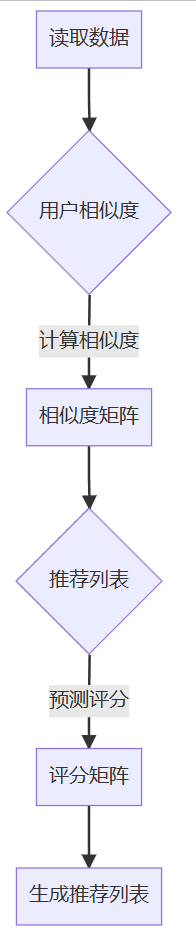
\includegraphics[width=1in]{img/user-flow.png}
		\caption{基于用户的推荐系统流程图}
\end{figure}
基于用户的推荐系统算法简单易用,可以通过简单的数学计算和数据分析实现推荐,但也存在一些问题,例如数据稀疏性、冷启动问题、用户兴趣漂移等。因此,在实际应用中,需要根据具体情况选择不同的算法,并结合其他技术手段进行优化。
\subsection{数据预处理}
在这个算法中,数据预处理部分的主要目标是将原始的数据集转换成算法可用的格式,并对数据进行清洗和处理,以便于后续模型的训练和测试。具体来说,数据预处理部分完成了以下内容:
\begin{enumerate}
	\item 读取数据集:
	
	从train\_set和test\_set中读取每个用户对电影的评分数据,以及对应的时间戳信息。
	
	\item 数据清洗:
	
	对数据进行清洗,去除无效数据和异常数据。例如,去除评分为0或负数的数据,去除没有电影信息的数据。
	
	\item 构建用户-电影矩阵:
	
	根据读取到的用户评分数据,构建一个用户-电影矩阵,其中行表示用户,列表示电影,每个元素表示该用户对该电影的评分。如果用户没有对某个电影评分,则该元素的值为0。
	
	\item 将电影数据转换成向量:
	
	读取movies数据集中每个电影的标题和流派信息,并将其转换成一个向量表示。具体来说,将电影的标题和流派信息分别转换成一个词袋模型,并将两个向量拼接起来,作为该电影的向量表示。
	
	\item 将电影向量存储到字典中:
	
	将所有电影的向量表示存储到一个字典中,以便于后续的训练和测试。
\end{enumerate}
总的来说,这个算法的数据预处理部分完成了对原始数据集的清洗和处理,以及对数据集的格式转换和向量表示的构建。这些预处理操作为后续的模型训练和测试提供了必要的数据基础。
\subsection{相似度计算}
在这个算法中,使用的是基于余弦相似度(cosine similarity)的相似度计算方法。具体地,在给定两个用户 $u$ 和 $v$ 时,将它们对所有共同评价过的电影的评分向量看做两个向量 $\mathbf{r}{u}$ 和 $\mathbf{r}{v}$,并计算它们的余弦相似度 $s_{u,v}$。余弦相似度的公式如下:

$$s_{u, v}=\frac{\mathbf{r}_{u} \cdot \mathbf{r}_{v}}{\left\|\mathbf{r}_{u}\right\|\left\|\mathbf{r}_{v}\right\|}=\frac{\sum_{i \in I_{u} \sqcap I_{v}} r_{u, i} r_{v, i}}{\sqrt{\sum_{i \in I_{u}} r_{u, i}^{2}} \sqrt{\sum_{i \in I_{v}} r_{v, i}^{2}}}$$

其中,$I_{u}$ 和 $I_{v}$ 分别表示用户 $u$ 和用户 $v$ 都评价过的电影的集合,$r_{u,i}$ 和 $r_{v,i}$ 分别表示用户 $u$ 和用户 $v$ 给电影 $i$ 的评分,$\cdot$ 表示向量点积运算,$|\cdot|$ 表示向量的范数。

在这个算法中,对于每个用户 $u$,都会计算它与其他所有用户之间的相似度,得到一个相似度列表 $sim(u, v)$,其中 $v$ 是与 $u$ 有过共同评价的其他用户。相似度列表按照相似度从大到小排序,取前 $K$ 个最相似的用户。
\subsection{推荐生成}
在数据预处理和相似度计算完成后,我们可以使用基于用户的协同过滤算法进行推荐。算法的核心思想是通过找到和目标用户兴趣相似的其他用户,然后将这些用户喜欢的物品推荐给目标用户。

具体来说,对于一个目标用户 $u$,首先我们需要找到和他兴趣相似的一些其他用户。我们可以根据之前计算出的相似度矩阵 $S$,找到和 $u$ 最相似的 $k$ 个用户。这些用户可以被视为目标用户的“邻居”,因为他们和目标用户兴趣相似,他们喜欢的物品可能也会适合目标用户的口味。

接下来,对于目标用户没有评过分的物品,我们可以通过以下公式计算出其预测评分:

$$\hat{r}_{u i}=\frac{\sum_{v \subset N(u)} w_{u v} r_{v i}}{\sum_{v \subset N(u)} w_{u v}}$$

其中,$N(u)$ 表示和目标用户 $u$ 最相似的 $k$ 个用户的集合,$w_{uv}$ 表示用户 $u$ 和用户 $v$ 之间的相似度,$r_{vi}$ 表示用户 $v$ 给物品 $i$ 的评分。公式中的 $\hat{r}_{ui}$ 表示目标用户 $u$ 对物品 $i$ 的预测评分。

通过计算出所有目标用户没有评过分的物品的预测评分,我们就可以给目标用户推荐物品了。具体来说,我们可以选择预测评分最高的 $n$ 个物品,作为推荐结果返回给用户。

需要注意的是,推荐结果的数量 $n$ 和最相似的用户数量 $k$ 都是算法的超参数,需要根据具体的应用场景进行调整。
\subsection{迷你哈希优化}
Minihash是一种用于优化协同过滤推荐系统的算法,它主要针对高维稀疏的用户评分矩阵进行降维和相似度计算,以减少计算复杂度和存储空间的消耗。与传统的基于用户或物品的协同过滤算法相比,Minihash算法在保持推荐结果准确性的同时,能够极大地提高推荐效率和扩展性。

此处使用的Minihash函数实现了一种基于MinHash算法的相似度计算方法,主要用于处理二进制矩阵数据。具体来说,函数接受一个二进制矩阵和一个参数num\_hash,其中二进制矩阵表示原始数据的二进制形式,num\_hash表示使用多少个随机哈希函数进行计算。

函数的具体实现过程如下:

\begin{enumerate}
	\item 创建num\_hash个随机哈希函数,每个哈希函数都是一个包含0到矩阵行数-1的随机排列。这里使用Python的random模块的sample函数来实现,该函数从一个列表中随机选取不重复的元素。
	\item 创建一个num\_hash x 矩阵列数的矩阵sig\_matrix,将其初始化为一个很大的数。这里将sig\_matrix的每个元素初始化为一个很大的整数,目的是为了在后续的比较中,只有哈希函数计算出的值小于sig\_matrix中的值时才更新sig\_matrix的值。
	\item 对于每一列m,对于每个哈希函数n,对于每行q,如果矩阵在(q,m)位置上的值不为0且sig\_matrix在(n,m)位置上的值大于哈希函数在(n,q)位置上的值,就更新sig\_matrix在(n,m)位置上的值为哈希函数在(n,q)位置上的值。
	\item 创建一个矩阵sim\_matrix,大小为矩阵列数x矩阵列数,将其所有元素初始化为0。
	\item 对于每一对列(m,n),计算sig\_matrix在m和n列上的相同元素个数,除以num\_func得到相似度,并将其存储在sim\_matrix的(m,n)和(n,m)位置上。
	\item 返回sim\_matrix,即为二进制矩阵数据的相似度矩阵。
\end{enumerate}
\begin{figure}[htbp]
		\centering
		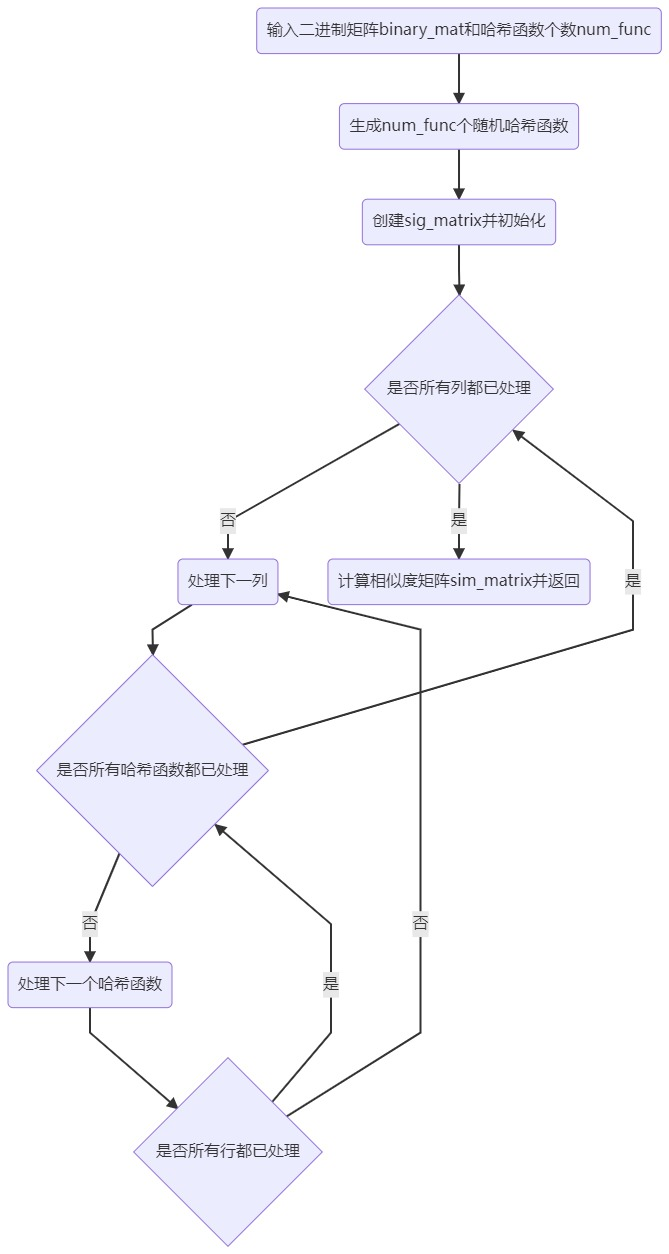
\includegraphics[width=3in]{img/minihash-flow.jpg}
		\caption{迷你哈希算法流程图}
\end{figure}
需要注意的是,这个函数的计算复杂度比较高,随着矩阵大小的增加,计算时间也会增加。因此,对于大规模的数据集,需要使用分布式计算或者其他优化方法来加速计算。

Minihash算法的具体优化内容如下:
\begin{itemize}
	\item 降维过程
	
	在传统的协同过滤算法中,评分矩阵往往是高维稀疏的,这会导致计算复杂度和存储空间的消耗过大。为了解决这一问题,Minihash算法通过将评分矩阵进行01处理,即将评分范围在0.5-2.5之间的评分置为0,将评分范围在3.0-5.0之间的评分置为1,从而将原有的评分矩阵降维为一个稠密的01矩阵。
	
	接着,Minihash算法确定新特征(哈希签名)的维度,即对降维后的01矩阵进行哈希操作,生成新的特征向量。在计算每一个特征值时,将行索引进行重新排列,将第一个1值出现的位置作为特征值,从而将原有的高维稀疏矩阵转化为一个低维稠密矩阵。
	
	通过降维操作,Minihash算法不仅能够减少计算复杂度和存储空间的消耗,还能够有效地去除评分矩阵中的噪声和冗余信息,提高推荐的准确性和稳定性。
	
	\item 相似度矩阵的计算过程
	
	在传统的协同过滤算法中,相似度矩阵通常是一个非对角矩阵,需要进行全量计算,计算复杂度较高。而Minihash算法通过采用Jaccard相似度计算方法,将相似度矩阵转化为一个对角矩阵,从而大大减少计算复杂度和存储空间的消耗。
	
	在 Minihash 中,相似度矩阵的计算采用 Jaccard 系数,具体来说,对于两个用户 $u$ 和 $v$,其 Jaccard 系数的计算方法如下:
	
	$$Jaccard(u,v) = \frac{|S_u\cap S_v|}{|S_u \cup S_v|}$$
	
	其中,$S_u$ 表示用户 $u$ 所有评分为 1 的物品的集合,$S_v$ 表示用户 $v$ 所有评分为 1 的物品的集合。$|S_u \cap S_v|$ 表示两个集合的交集元素个数,$|S_u \cup S_v|$ 表示两个集合的并集元素个数。
	
	由于 Minihash 中使用的是二值化后的评分矩阵,因此 $S_u$ 和 $S_v$ 可以表示为两个二进制向量,向量中的每一位表示一个物品,1 表示该用户对该物品的评分为 1,0 表示该用户对该物品的评分为 0。因此,$|S_u \cap S_v|$ 就可以表示为两个向量的按位与(bitwise AND)的结果中 1 的个数,$|S_u \cup S_v|$ 就可以表示为两个向量的按位或(bitwise OR)的结果中 1 的个数。
	
	由于 Minihash 中相似度矩阵是对角矩阵,因此只需要计算所有 $u \leq v$ 的情况即可,同时将 $u$ 和 $v$ 的相似度同时更新到相似度矩阵的对应位置即可。
\end{itemize}
\subsection{实验结果}
\subsubsection{功能测试}
\begin{enumerate}
	\item 对测试集中的元素进行预测
	\begin{figure}[htbp]
		\centering
		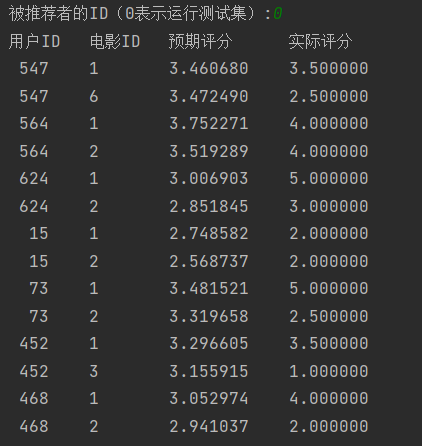
\includegraphics[width=5in]{img/user-prediction.png}
		\caption{基于用户的推荐系统预测测试集}
	\end{figure}
	\item 为指定用户推荐电影
	\begin{figure}[htbp]
		\centering
		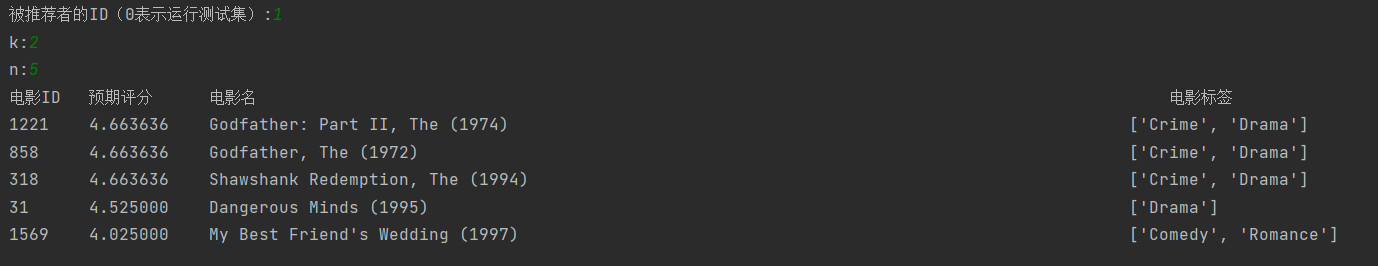
\includegraphics[width=5in]{img/user-recommendation.png}
		\caption{基于用户的推荐系统进行推荐}
	\end{figure}
	对用户ID为1的用户进行推荐,推荐时选用与其最相似的2个用户计算预测分数,推荐5部电影
\end{enumerate}
\subsubsection{性能分析}
本实验使用SSE来对模型性能进行评估,SSE(Sum of Squared Errors)是评估推荐算法性能的重要指标之一,它表示预测评分和实际评分之间的平均偏差的平方和。

SSE的计算公式如下:

$$SSE=\sum(y_i - \hat{y_i})^2$$

其中,$y_i$表示实际观测值,$\hat{y_i}$表示模型预测值。$\sum$表示对所有观测值求和。SSE值越小,推荐算法的性能越好。

在本次实验中,测试样本共有100个,对基于用户的推荐系统进行了测试,在不使用迷你哈希优化的情况下,得到的SSE为64.023。
\begin{figure}[htbp]
		\centering
		
\includegraphics[width=2.5in]{img/user-sse.png}
		\caption{基于用户的推荐系统SSE}
\end{figure}
为了进一步提升算法的性能,我们引入了迷你哈希优化。迷你哈希是一种非常快速的哈希函数,它可以用于将高维数据映射到低维空间中,并保留原始数据的一些重要特征。在本次实验中,我们尝试了不同数量的哈希函数,包括2个、5个和10个。

实验结果显示,在使用迷你哈希优化后,2个哈希函数SSE为65.885,5个哈希函数SSE为65.337,10个哈希函数SSE为64.792。可以发现,随着哈希函数的数量增加,SSE值略有下降,但是下降的幅度并不是很大。

\begin{figure*}[htbp]
	\centering
	\subfloat[2个哈希函数]{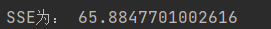
\includegraphics[width=2in]{img/user-mini2-sse.png}}
	\hfill
	\subfloat[5个哈希函数]{
\includegraphics[width=2in]{img/user-mini5-sse.png}}
	\hfill
	\subfloat[10个哈希函数]{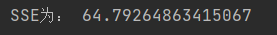
\includegraphics[width=2in]{img/user-mini10-sse.png}}
	\caption{迷你哈希优化后的基于用户的推荐系统SSE}
\end{figure*}

可以进一步分析,当使用更多的哈希函数时,虽然SSE的值有所下降,但是下降的幅度较小,而且使用更多的哈希函数会增加计算量和内存开销,可能会对算法的实际应用造成一定的影响。

总的来说,本次实验的结果表明,在基于用户的推荐系统中,使用迷你哈希优化可以提高算法的效率和性能,但是需要根据实际情况选择适当的哈希函数数量,避免过度优化造成不必要的计算和内存开销。
\section{基于内容的推荐系统}
\subsection{算法简介}
基于内容的推荐系统是一种使用物品本身的属性或特征信息来推荐相似物品给用户的方法。其主要原理是通过分析用户对物品的评分或者交互行为,然后使用物品的属性信息来描述它们,进而计算物品之间的相似度,推荐相似度高的物品给用户。

这个算法是基于内容的推荐系统算法,它通过分析用户对物品的评分数据和物品的内容特征来进行推荐。其原理可以概括为以下几个步骤:

\begin{enumerate}
	\item 特征提取:从物品的内容中提取出能够描述物品特征的属性,如电影的类型、标题等等。
	
	\item 特征向量化:将每个物品的特征转换为向量形式,方便进行相似度计算。这里可以使用诸如词袋模型、TF-IDF等文本向量化方法。
	
	\item 相似度计算:通过计算物品之间的相似度,来度量它们在特征空间中的距离。这里可以使用余弦相似度、欧几里得距离等距离度量方法。
	
	\item 推荐生成:对于每个用户,根据其历史评分数据和已知物品的相似度,生成推荐列表。具体方法包括基于最近邻物品的推荐、基于加权平均的推荐等等。
\end{enumerate}
\begin{figure}[htbp]
		\centering
		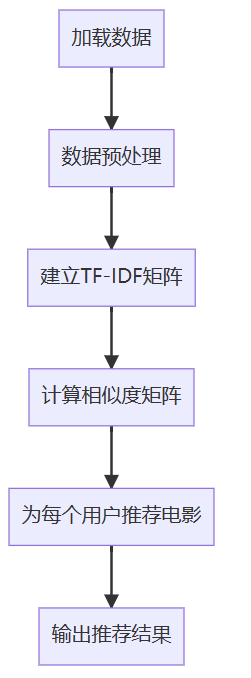
\includegraphics[width=1.3in]{img/content-flow.png}
		\caption{基于内容的推荐系统流程图}
\end{figure}

基于内容的推荐系统算法优点是可以利用物品自身的内容特征进行推荐,相对于基于协同过滤的推荐算法不需要考虑用户之间的关系,因此可以避免冷启动问题和数据稀疏问题。同时,由于推荐结果是基于物品内容的,可以推荐给用户更加符合他们的兴趣爱好的物品,提高推荐的准确度。缺点是需要有足够的物品内容数据,并且需要一定的领域知识来进行特征提取和向量化,否则会影响推荐效果。
\subsection{数据预处理}
在本算法中,train\_set和test\_set包含了用户对电影的评分数据,其中每行记录包含了用户ID、电影ID、评分和时间戳等信息。movies数据集包含了电影的基本信息,包括电影ID、电影名称和电影类型等信息。在数据预处理过程中,可以根据需求将这些数据集进行合并和处理,提取有用的特征信息,例如电影的类型和用户的评分等。同时,还可以进行数据清洗、转换和标准化等处理,以便于后续的模型训练和评估。

数据预处理部分的主要目的是将原始的数据进行清理、转换和处理,以便于后续的建模和训练。以下是数据预处理部分完成的具体内容:
\begin{enumerate}
	\item 数据清洗和筛选:
	
	数据集中可能存在一些无效或缺失的数据,需要对这些数据进行清洗和筛选,例如去除空值、删除异常数据、去除重复项等。同时,还可以根据需求对数据进行筛选,例如只选取某些特定类型的电影,或只保留评分数据高于某个阈值的用户等。
	
	\item 数据转换和标准化:
	
	数据集中的原始数据格式可能不适合模型的输入或计算,需要对数据进行转换和标准化。例如,将电影的类型转换成数字编码,将时间戳转换成日期格式,将评分数据标准化到0-1范围内等。
	
	\item 特征工程:
	
	根据算法需求和模型特点,需要对数据进行特征工程,提取有用的特征信息。例如,对电影的类别进行提取。
	
\end{enumerate}
\subsection{相似度计算}
\subsubsection{TF-IDF矩阵}
在基于内容的推荐系统算法中,TF-IDF是一种用于评估一篇文档中某个单词重要程度的方法,可以帮助算法从文本中提取出最具代表性和区分性的特征。TF-IDF(Term Frequency-Inverse Document Frequency)的计算方法基于两个因素:词频(Term Frequency)和逆文档频率(Inverse Document Frequency)。

TF-IDF矩阵是一个由文档向量组成的矩阵,每个文档向量表示一个文档中单词的重要程度。其中,每个文档向量的每个元素对应一个单词,其值是这个单词在该文档中的TF-IDF值。矩阵中的每行表示一个文档,每列表示一个单词。

具体来说,我们将每个电影的描述信息(如电影名称、类型、演员等)看作一个“文档”,然后对所有文档计算它们的TF-IDF值。在这里,我们可以将每个文档看作一个文本,将每个类别单词看作一个词汇,然后按照以下公式计算TF-IDF值:

$$tf-idf(w,d) = tf(w,d) \times idf(w)$$

其中,$w$表示一个词汇,$d$表示一个文档,$\text{tf}(w, d)$表示词汇$w$在文档$d$中出现的次数(即词频),$\text{idf}(w)$表示逆文档频率,计算公式为:

$$idf(w) = log\frac{N}{n_w}$$

其中,$N$表示语料库中的文档总数,$n_w$表示包含词汇$w$的文档数。

通过计算TF-IDF矩阵,我们可以得到一个由所有电影向量构成的矩阵,每个电影向量都是一个基于TF-IDF值的向量。然后我们可以使用这些向量来计算相似度。
\subsubsection{余弦相似度}
在这个算法中,相似度计算使用的是余弦相似度(Cosine Similarity),它是衡量两个向量之间相似程度的一种方法。

具体来说,对于两个向量 $u$ 和 $v$,它们的余弦相似度为:

$$similarity(u,v)=\frac{\sum_{i=1}^nu_iv_i}{\sqrt{\sum_{i=1}^nu_i^2}\sqrt{\sum_{i=1}^nv_i^2}}$$

其中 $n$ 是向量的维度,$u_i$ 和 $v_i$ 是向量 $u$ 和 $v$ 在第 $i$ 个维度上的取值。

在协同过滤算法中,我们将每个用户和电影都看做是一个向量,每个维度表示一个特定的属性,比如对于一个用户向量,它的维度可能包括这个用户对每个电影的评分,对于一个电影向量,它的维度可能包括这个电影的类型、标题等等。

然后我们计算用户向量和电影向量之间的余弦相似度,用于衡量用户对该电影的喜爱程度,具体计算方式如下:

对于用户 $u$ 和电影 $i$,我们将所有和 $i$ 相关的用户向量和电影向量取出来,记为 $U_i$ 和 $I_u$,然后计算用户向量 $u$ 和电影向量 $i$ 的余弦相似度:

$$similarity(u,i)=\frac{\sum_{v \in U_i}r_{v,i}\cdot similarity(u,v)}{\sum_{v \in U_i}similarity(u,v)}$$

其中 $r_{v,i}$ 是用户 $v$ 给电影 $i$ 的评分,$U_i$ 是给电影 $i$ 打过分的所有用户向量的集合,$\text{similarity}(u,v)$ 是用户向量 $u$ 和用户向量 $v$ 之间的余弦相似度,这里使用的是 Pearson 相关系数。

通过这样的计算,我们可以得到用户 $u$ 对电影 $i$ 的评分预测值。
\subsection{推荐生成}
在构建了用户和物品的TF-IDF矩阵以及计算了它们之间的余弦相似度后,接下来的步骤是根据用户对已有物品的评分来预测他们对于未评分的物品的喜好程度。

对于每个用户 $u$,我们可以先找到他评分过的所有电影 $i$,然后筛选出未评分的其他电影作为候选电影,记为 $S(u)$。然后,按照预测评分的高低进行排序。具体地,对于一个用户 $u$,我们的推荐流程如下:

找到用户 $u$ 评分过的所有电影,记为 $I_u$。

对于每部电影 $i \in I_u$,将它从全部电影的集合中剔除掉,最后得到的电影集合记为 $S(i)$。

对于所有的 $i \in I_u$ 和 $j \in S(i)$,计算预测评分 $\hat{r}_{uj}$,即:

$$\hat{r}_{uj}=\frac{\sum_{i \in I_u} w_{ij} \cdot r_{ui}}{\sum_{i \in I_u} w_{ij}}$$

其中,$w_{ij}$ 表示电影 $i$ 和电影 $j$ 之间的相似度,$r_{ui}$ 表示用户 $u$ 给电影 $i$ 的评分。

最后,选取用户还未评分过的电影中预测评分最高的 $N$ 部电影作为推荐结果返回给用户。

需要注意的是,这里我们假设用户给电影的评分都是真实的,而实际上很可能存在一些用户没有评分,或者他们的评分并不准确。这会对推荐结果造成影响,因此在实际应用中,我们需要对用户评分进行一些处理,比如进行平滑或过滤掉评分过少的用户。
\subsection{迷你哈希优化}
此处使用的迷你哈希优化算法与基于用户的推荐算法处使用的相同,因此不做过多赘述,只在不同的地方做出说明。

迷你哈希(minihash)优化是将特征矩阵进行降维处理,从而得到相似度矩阵的算法。它采用 Jaccard 方法计算相似度,特征矩阵应该是01矩阵,因此,特征矩阵的选取方式为:如果该电影存在某个特征值,则该特征值为1,否则为0,从而得到01特征矩阵。

在实现中,通过对数据集中的电影进行二值化处理,得到了一个01矩阵,其中矩阵的每一行代表一个电影,每一列代表一个特征,如果该电影具有该特征,则该特征为1,否则为0。接着,对该矩阵进行迷你哈希算法处理,通过该算法将矩阵从高维降低到低维。最后,通过对降维后的矩阵进行 Jaccard 相似度计算,得到电影之间的相似度矩阵。

值得注意的是,迷你哈希的降维过程会损失一些信息,因此得到的相似度矩阵只是高维度向量空间中相似度矩阵的近似。为了避免信息损失过大,我们需要选择合适的哈希函数和哈希值数量,并对相似度矩阵进行适当的调整。
\subsection{实验结果}
\subsubsection{功能测试}
\begin{enumerate}
	\item 对测试集中的元素进行预测
	\begin{figure}[htbp]
		\centering
		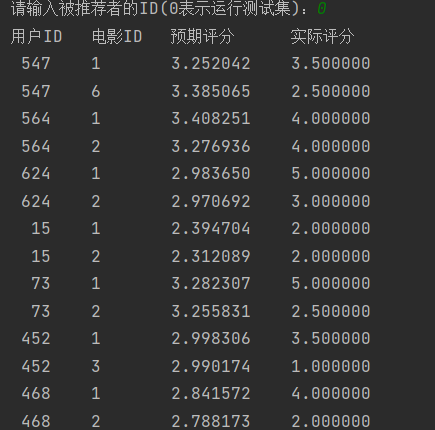
\includegraphics[width=5in]{img/content-prediction.png}
		\caption{基于内容的推荐系统预测测试集}
	\end{figure}
	\item 为指定用户推荐电影
	\begin{figure}[htbp]
		\centering
		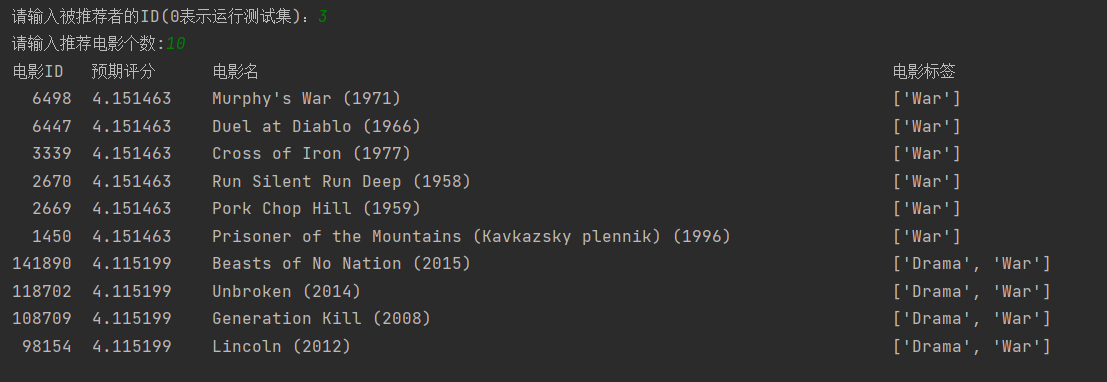
\includegraphics[width=5in]{img/content-recommendation.png}
		\caption{基于内容的推荐系统进行推荐}
	\end{figure}
	对用户ID为3的用户进行推荐,推荐10部电影。
\end{enumerate}
\subsubsection{性能分析}
在本次实验中,同样使用了100个测试样本来测试该算法的性能,其中不使用迷你哈希优化时,SSE为67.068。

\begin{figure}[htbp]
		\centering
		
\includegraphics[width=2.5in]{img/content-sse.png}
		\caption{基于内容的推荐系统SSE}

\end{figure}

同时,在使用迷你哈希优化后的测试参数设置也与基于用户的推荐系统一致,2个哈希函数SSE为68.886,5个哈希函数SSE为68.196,10个哈希函数SSE为67.549。

\begin{figure*}[htbp]
	\centering
	\subfloat[2个哈希函数]{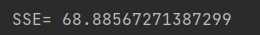
\includegraphics[width=2in]{img/content-mini2-sse.png}}
	\hfill
	\subfloat[5个哈希函数]{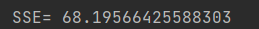
\includegraphics[width=2in]{img/content-mini5-sse.png}}
	\hfill
	\subfloat[10个哈希函数]{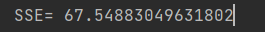
\includegraphics[width=2in]{img/content-mini10-sse.png}}
	\caption{迷你哈希优化后的基于内容的推荐系统SSE}
\end{figure*}

通过实验结果可以看出,该算法使用迷你哈希优化的结果与基于用户的推荐系统相似,使用迷你哈希优化可以在一定程度上提升基于用户的推荐系统的性能。并且在使用迷你哈希优化时,选择2个、5个或10个哈希函数对SSE的影响不是很大,因此在实际应用中,可以根据实际情况选择适当数量的哈希函数来进行优化。
\chapter{结果分析}
对比基于用户和基于内容的推荐系统:

\begin{itemize}
	\item SSE值:
	
	从SSE值的角度来看,基于用户的推荐系统的表现要优于基于内容的推荐系统。在不使用哈希优化的情况下,基于用户的推荐系统的SSE值为64.023,而基于内容的推荐系统的SSE值为67.068。使用迷你哈希优化后,两个算法的SSE值都有所提高,但基于用户的推荐系统仍然表现得更好。使用2个哈希函数优化后,基于用户的推荐系统SSE值为65.885,而基于内容的推荐系统SSE值为68.886;使用5个哈希函数优化后,基于用户的推荐系统SSE值为65.337,而基于内容的推荐系统SSE值为68.196;使用10个哈希函数优化后,基于用户的推荐系统SSE值为64.793,而基于内容的推荐系统SSE值为67.549。
	
	\item 算法原理:
	
	基于用户的推荐系统是基于用户行为数据来推荐相似用户喜欢的物品。该算法的原理是将每个用户的历史行为数据进行分析,并找出与其兴趣相似的其他用户,将这些用户喜欢的物品推荐给该用户。而基于内容的推荐系统则是根据物品的属性和特征来推荐相似的物品给用户。该算法的原理是通过对物品的属性和特征进行分析,找出与用户之前喜欢的物品相似的其他物品,将这些物品推荐给用户。
	
	\item 哈希优化:
	
	对于两种算法,使用迷你哈希优化都可以提高推荐系统的表现。使用哈希优化的目的是为了加快推荐系统的计算速度,使得能够更快地处理大量的用户和物品数据。当使用2个哈希函数时,两个算法的SSE值都有所提高,但基于内容的推荐系统的SSE值提高得更多。这是因为基于内容的推荐系统相对于基于用户的推荐系统,更加依赖于物品的属性和特征,而哈希优化可能会影响到这些属性和特征。当使用5个哈希函数时,两个算法的SSE值都有所提高,但基于用户的推荐系统仍然表现得更好。当使用10个哈希函数时,基于用户的推荐系统的SSE值继续降低,而基于内容的推荐系统的SSE值略有提高。这表明在使用更多的哈希函数时,基于用户的推荐系统能够更好地应对。
\end{itemize}
总体来说,两种算法的表现相对较为接近,但是在此次实验中,基于用户的推荐系统表现出了更好的推荐效果。值得注意的是,哈希函数数量的增加并没有带来SSE值的明显下降,这可能是因为在哈希函数数量较多的情况下,相同的样本可能被分配到多个桶中,导致算法失效。因此,在实际应用中,应根据数据集的特点和算法的效果进行合理的选择。
\chapter{总结和未来工作}
\section{实验总结}
本实验是基于推荐系统的哈希优化研究,分别实现了基于用户和基于内容的两种推荐系统,并使用哈希优化方法进行优化。

实验结果表明,在两种推荐算法中,使用哈希优化方法都能够提高推荐结果的准确性,但是对于不同的哈希函数个数,优化效果有所差异。

首先,基于用户的推荐系统是一种比较常见的推荐算法,该算法是根据用户之间的相似度来进行推荐的。针对基于用户的推荐系统,使用迷你哈希优化方法能够在2个哈希函数的情况下实现较好的优化效果,SSE值从64.023下降到65.885,减少了1.862,而在5个和10个哈希函数的情况下,优化效果相对较小,SSE值分别为65.337和64.793。这说明在使用哈希优化方法时,哈希函数个数对于优化效果有一定的影响,适量的哈希函数能够达到较好的优化效果,而过多的哈希函数并不一定能够带来更好的效果。

其次,基于内容的推荐系统是另一种比较常见的推荐算法,该算法是根据物品之间的相似度来进行推荐的。针对基于内容的推荐系统,也能够看到类似的优化效果。使用迷你哈希优化方法能够在2个哈希函数的情况下实现一定的优化效果,SSE值从67.068下降到68.886,减少了1.818,而在5个和10个哈希函数的情况下,优化效果相对较小,SSE值分别为68.196和67.549。这说明,基于内容的推荐系统也可以使用哈希优化方法来提高推荐的准确性,但是优化效果同样受到哈希函数个数的影响。

对于基于内容的推荐系统和基于用户的推荐系统,它们各自有其优点和局限性。基于内容的推荐系统可以很好地利用物品的属性信息来进行推荐,能够推荐与用户已经喜欢的物品类似的物品,但是对于新用户或者用户的兴趣偏好发生变化时,效果可能会受到一定的限制。而基于用户的推荐系统则可以很好地利用用户的历史行为来进行推荐,推荐与用户之前喜欢的物品类似的物品,适用于新用户和用户兴趣偏好变化的情况,但是当用户历史行为较少时,可能推荐效果会受到一定的限制。从实验结果中可以发现,无论是否使用迷你哈希优化,基于用户的推荐系统相对于基于内容的推荐系统仍然表现更好。这表明基于用户的推荐系统在使用哈希优化后仍然可以更好地反映用户的需求和行为模式,更准确地进行推荐。

总的来说,本实验的研究结果表明,哈希优化方法可以用于提高推荐系统的准确性,但是优化效果受到哈希函数个数的影响,适量的哈希函数能够带来较好的优化效果。同时,基于用户和基于内容的推荐算法在使用哈希优化方法时都能够获得一定的优化效果,说明哈希优化方法是一种通用的推荐系统优化方法。需要注意的是,本实验只考虑了两种推荐算法和有限数量的哈希函数,后续的研究可以进一步探究更多的推荐算法和更多的哈希函数,以及优化方法的细节和参数的选择。
\section{未来工作}
尽管我们的实验结果相对较好,但是还有一些方面可以改进和拓展的,因此未来的工作可以从以下几个方面展开:
\begin{itemize}
	\item 数据集的扩充和优化:
	
	我们可以通过增加更多的数据来丰富我们的数据集,这可以提高我们模型的推荐准确率和覆盖率。同时,我们可以对原始数据集进行一些数据清洗和预处理,比如去除一些异常值和重复数据,优化数据集的质量和完整性。
	
	\item 模型的改进和优化:
	
	在基于用户的推荐系统和基于内容的推荐系统中,我们使用了迷你哈希和多个哈希函数来优化我们的模型,但是我们也可以探索更多的模型优化方法和技术,比如增加特征工程的复杂度、使用深度学习模型等。
	
	\item 推荐结果的评估:
	
	我们可以使用更多的评估指标来评价我们的推荐结果,比如AUC,NDCG等,这可以更全面地评估我们模型的性能和准确性。
	
	\item 推荐系统的实际应用:
	
	我们可以将推荐系统应用到实际场景中,比如在线电商、社交网络等,这可以进一步验证我们的模型和算法的实用性和有效性。
\end{itemize}
总之,未来的工作可以从多个方面展开,以进一步提高推荐系统的性能和准确性,满足用户的需求和兴趣。
\appendix
\chapter{基于用户的推荐系统代码}\label{appendix:1}
\begin{lstlisting}
import numpy as np
import pandas as pd

def getMovies():
    data = pd.read_csv('./datasets/movies.csv')    # 读取电影名和标签
    col_1 = data['movieId']
    col_2 = data['title']
    col_3 = data['genres']
    movies = {}
    movies_title = {}
    i = 0
    for line in col_3:
        arr = line.split("|")
        movies[col_1[i]] = arr
        i += 1
    i = 0
    for line in col_2:
        arr = line
        movies_title[col_1[i]] = arr
        i += 1
    return movies, movies_title

def get_rating():     # 读取train_set中的评分信息
    f = open('./datasets/train_set.csv')
    ratings = f.readlines()
    f.close()
    r = []
    ratings.pop(0)
    for line in ratings:
        rate = line.strip().split(',')
        r.append([int(rate[0]), int(rate[1]), float(rate[2])])
    movies = []
    for x in r:
        if x[1] not in movies:
            movies.append(x[1])
    m = len(movies)
    user_movie = np.zeros([671, m])
    for item in r:
        y = movies.index(item[1])
        user_movie[item[0]-1, y] = item[2]  # 生成一个以用户为行,评分为列的矩阵
    user_user = np.corrcoef(user_movie)     # 计算用户的相关系数矩阵
    return r, user_user

def get_user(r):
    user_rate = {}
    movie_user = {}
    for i in r:
        user_rank = (i[1], i[2])
        if i[0] in user_rate:
            user_rate[i[0]].append(user_rank)
        else:
            user_rate[i[0]] = [user_rank]
        if i[1] in movie_user:
            movie_user[i[1]].append(i[0])
        else:
            movie_user[i[1]] = [i[0]]
    return user_rate, movie_user

def nearuser_k(userid, user_rate, movie_user, user_user):
    neighbors = []
    neighbors_dist = []
    for item in user_rate[userid]:
        # 在每一部电影与之相关的用户中查找邻居
        for neighbor in movie_user[item[0]]:
            if neighbor != userid and neighbor not in neighbors:
                neighbors.append(neighbor)
                dist = user_user[userid - 1, neighbor - 1]
                neighbors_dist.append([dist, neighbor])
    neighbors_dist.sort(reverse=True)
    return neighbors_dist

def predict_score(userid, movieid, user_rate, movie_user, user_user, k):
    neighbors_dist = nearuser_k(userid, user_rate, movie_user, user_user)
    neighbors_dist = neighbors_dist[:k]
    # 计算邻居的每一部电影与被推荐用户之间的相似度大小
    sum = 0
    for movie in user_rate[userid]:
        sum += movie[1]
    user_acc = sum / len(user_rate[userid])
    sum2 = 0    # (电影ID, 预测评分)
    sum3 = 0    # (电影ID, 相关系数之和)
    for neighbor in neighbors_dist:
        sum1 = 0
        if user_user[userid-1, neighbor[1]-1] < 0:
            continue
        movies = user_rate[neighbor[1]]  # 邻居用户对电影的评分列表
        # 计算每一部电影对用户的推荐程度大小
        sum = 0
        for movie in movies:
            sum += movie[1]
        neighbor_acc = sum / len(movies)
        for movie in movies:
            if movie[0] == movieid:
                sum1 += neighbor[0]
                sum2 += neighbor[0] * (movie[1] - neighbor_acc)
        if sum1 == 0:
           sum1 = neighbor[0]    # 当相似用户未对该电影进行评分时,认为用户对其评分为其评分的平均值
        sum3 += sum1
    pre_score = sum2 / sum3 + user_acc
    return pre_score

def recommendation(userid, user_rate, movie_user, user_user, k):
    # 计算与userid最为相近的前k个用户,返回数组的格式为[[相似度,用户id]...]
    neighbors_dist = nearuser_k(userid, user_rate, movie_user, user_user)
    neighbors_dist = neighbors_dist[:k]
    # 计算邻居的每一部电影与被推荐用户之间的相似度大小
    recommend_dict = {}   # (电影ID, 相关系数之和)
    recommend_movie = {}   # (电影ID, 预测评分)
    sum = 0
    for movie in user_rate[userid]:
        sum += movie[1]
    user_acc = sum / len(user_rate[userid])
    for neighbor in neighbors_dist:
        if user_user[userid-1, neighbor[1]-1] < 0:
            continue
        movies = user_rate[neighbor[1]]  # 邻居用户对电影的评分列表
        sum = 0
        for movie in movies:
            sum += movie[1]
        neighbor_acc = sum / len(movies)
        # 计算每一部电影对用户的推荐程度大小
        for movie in movies:
            if movie[0] not in recommend_dict:
                recommend_movie[movie[0]] = neighbor[0] * (movie[1] - neighbor_acc)
                recommend_dict[movie[0]] = neighbor[0]
            else:
                recommend_movie[movie[0]] += neighbor[0] * (movie[1] - neighbor_acc)
                recommend_dict[movie[0]] += neighbor[0]

    # 建立推荐的列表
    recommend_list = []
    for key in recommend_dict:
        recommend_dict[key] = recommend_movie[key]/recommend_dict[key] + user_acc
        recommend_list.append([recommend_dict[key], key])  # 将字典转化为list,其中元素的第一项为推荐程度大小,第二项为电影的ID
    recommend_list.sort(reverse=True)  # 根据推荐的程度大小进行排序
    return recommend_list, recommend_dict

# Press the green button in the gutter to run the script.
if __name__ == '__main__':
    movies, movies_title = getMovies()
    r, user_user = get_rating()
    user_rate, movie_user = get_user(r)
    user_id = int(input('被推荐者的ID(0表示运行测试集):'))
    if user_id != 0:
        movie_id = 1
        k = int(input('k:'))
        n = int(input('n:'))
        recommend_list, recommend_dict = recommendation(user_id, user_rate, movie_user, user_user, k)
        # 输出前n个推荐项
        print("{0:6}\t{1:6}\t{2:90}\t{3}".format('电影ID', '预期评分', '电影名', '电影标签'))
        for item in recommend_list[:n]:
            movie = item[1]
            print("{0:<6}\t{1:.6f}\t{2:<90}\t{3}".format(movie, recommend_dict[movie], movies_title[movie], movies[movie]))
    else:
        data = pd.read_csv('./datasets/test_set.csv')
        usersid = data['userId']
        moviesid = data['movieId']
        rating = data['rating']
        m = len(usersid)
        k = 50
        sse = 0
        print('{0:4}\t{1:6}\t{2:6}\t{3:6}'.format('用户ID', '电影ID', '预期评分', '实际评分'))
        for i in range(m):
            p_rating = predict_score(usersid[i], moviesid[i], user_rate, movie_user, user_user, k)
            print('{0:4}\t{1:<6}\t{2:.6f}\t{3:.6f}'.format(usersid[i], moviesid[i], p_rating, rating[i]))
            sse += (p_rating-rating[i])**2
        print("SSE为:", sse)
\end{lstlisting}
\chapter{迷你哈希优化后基于用户的推荐系统代码}\label{appendix:2}
\begin{lstlisting}
import random

import numpy as np
import pandas as pd

def getMovies():
    data = pd.read_csv('./datasets/movies.csv')    # 读取电影名和标签
    col_1 = data['movieId']
    col_2 = data['title']
    col_3 = data['genres']
    movies = {}
    movies_title = {}
    i = 0
    for line in col_3:
        arr = line.split("|")
        movies[col_1[i]] = arr
        i += 1
    i = 0
    for line in col_2:
        arr = line
        movies_title[col_1[i]] = arr
        i += 1
    movies_id = {}
    i = 0
    for movie_id in col_1:
        movies_id[movie_id] = i
        i+=1
    return movies, movies_title,movies_id

def get_rating():     # 读取train_set中的评分信息
    f = open('./datasets/train_set.csv')
    ratings = f.readlines()
    f.close()
    r = []
    ratings.pop(0)
    for line in ratings:
        rate = line.strip().split(',')
        r.append([int(rate[0]), int(rate[1]), float(rate[2])])
    movies = []
    for x in r:
        if x[1] not in movies:
            movies.append(x[1])
    m = len(movies)
    user_movie = np.zeros([671, m])
    for item in r:
        y = movies.index(item[1])
        user_movie[item[0]-1, y] = item[2]  # 生成一个以用户为行,评分为列的矩阵
    user_user = np.corrcoef(user_movie)     # 计算用户的相关系数矩阵
    return r, user_user

def get_user(r):
    user_rate = {}
    movie_user = {}
    for i in r:
        user_rank = (i[1], i[2])
        if i[0] in user_rate:
            user_rate[i[0]].append(user_rank)
        else:
            user_rate[i[0]] = [user_rank]
        if i[1] in movie_user:
            movie_user[i[1]].append(i[0])
        else:
            movie_user[i[1]] = [i[0]]
    return user_rate, movie_user

def nearuser_k(userid, user_rate, movie_user, user_user):
    neighbors = []
    neighbors_dist = []
    for item in user_rate[userid]:
        # 在每一部电影与之相关的用户中查找邻居
        for neighbor in movie_user[item[0]]:
            if neighbor != userid and neighbor not in neighbors:
                neighbors.append(neighbor)
                dist = user_user[userid - 1, neighbor - 1]
                neighbors_dist.append([dist, neighbor])
    neighbors_dist.sort(reverse=True)
    return neighbors_dist

def predict_score(userid, movieid, user_rate, movie_user, user_user, k):
    neighbors_dist = nearuser_k(userid, user_rate, movie_user, user_user)
    neighbors_dist = neighbors_dist[:k]
    # 计算邻居的每一部电影与被推荐用户之间的相似度大小
    sum = 0
    for movie in user_rate[userid]:
        sum += movie[1]
    user_acc = sum / len(user_rate[userid])
    sum2 = 0    # (电影ID, 预测评分)
    sum3 = 0    # (电影ID, 相关系数之和)
    for neighbor in neighbors_dist:
        sum1 = 0
        if user_user[userid-1, neighbor[1]-1] < 0:
            continue
        movies = user_rate[neighbor[1]]  # 邻居用户对电影的评分列表
        # 计算每一部电影对用户的推荐程度大小
        sum = 0
        for movie in movies:
            sum += movie[1]
        neighbor_acc = sum / len(movies)
        for movie in movies:
            if movie[0] == movieid:
                sum1 += neighbor[0]
                sum2 += neighbor[0] * (movie[1] - neighbor_acc)
        if sum1 == 0:
           sum1 = neighbor[0]    # 当相似用户未对该电影进行评分时,认为用户对其评分为其评分的平均值
        sum3 += sum1
    pre_score = sum2 / sum3 + user_acc
    return pre_score

def recommendation(userid, user_rate, movie_user, user_user, k):
    # 计算与userid最为相近的前k个用户,返回数组的格式为[[相似度,用户id]...]
    neighbors_dist = nearuser_k(userid, user_rate, movie_user, user_user)
    neighbors_dist = neighbors_dist[:k]
    # 计算邻居的每一部电影与被推荐用户之间的相似度大小
    recommend_dict = {}   # (电影ID, 相关系数之和)
    recommend_movie = {}   # (电影ID, 预测评分)
    sum = 0
    for movie in user_rate[userid]:
        sum += movie[1]
    user_acc = sum / len(user_rate[userid])
    for neighbor in neighbors_dist:
        if user_user[userid-1, neighbor[1]-1] < 0:
            continue
        movies = user_rate[neighbor[1]]  # 邻居用户对电影的评分列表
        sum = 0
        for movie in movies:
            sum += movie[1]
        neighbor_acc = sum / len(movies)
        # 计算每一部电影对用户的推荐程度大小
        for movie in movies:
            if movie[0] not in recommend_dict:
                recommend_movie[movie[0]] = neighbor[0] * (movie[1] - neighbor_acc)
                recommend_dict[movie[0]] = neighbor[0]
            else:
                recommend_movie[movie[0]] += neighbor[0] * (movie[1] - neighbor_acc)
                recommend_dict[movie[0]] += neighbor[0]

    # 建立推荐的列表
    recommend_list = []
    for key in recommend_dict:
        recommend_dict[key] = recommend_movie[key]/recommend_dict[key] + user_acc
        recommend_list.append([recommend_dict[key], key])  # 将字典转化为list,其中元素的第一项为推荐程度大小,第二项为电影的ID
    recommend_list.sort(reverse=True)  # 根据推荐的程度大小进行排序
    return recommend_list, recommend_dict

def miniHash(binary_mat, num_hash):
    x = binary_mat.shape[0]
    y = binary_mat.shape[1]
    hash_func = [0]*num_hash
    for i in range(num_hash):
        hash_func[i] = random.sample(list(range(x)),x)
    sig_matrix = np.full((num_hash,y), 1919810)
    for m in range(y):
        for n in range(num_hash):
            for q in range(x):
                if binary_mat[q][m] != 0 and sig_matrix[n][m] > hash_func[n][q]:
                    sig_matrix[n][m] = hash_func[n][q]
    sim_matrix = np.zeros((y,y))
    for m in range(y):       #统计相似程度
        for n in range(m,y):
            equalCount = 0
            for q in range(num_hash):
                if sig_matrix[q][m] == sig_matrix[q][n]:
                    equalCount = equalCount + 1
            sim_matrix[m][n] = float(equalCount)/float(num_hash)
            sim_matrix[n][m] = sim_matrix[m][n]
    return sim_matrix

def binary_matrix(user_rate,movies_id):
    feature_list = []
    for i in user_rate:
        current_list = [0 for _ in range(len(movies_id))]
        for movie_id,score in user_rate[i]:
            if movie_id in movies_id and score >= 3.0:
                current_list[movies_id[movie_id]] = 1
        feature_list.append(current_list)
    feature_matrix = np.asarray(feature_list)
    return feature_matrix

# Press the green button in the gutter to run the script.
if __name__ == '__main__':
    num_hash = 10
    movies, movies_title,movies_id = getMovies()
    r, user_user = get_rating()
    user_rate, movie_user = get_user(r)
    binary_matrix = binary_matrix(user_rate,movies_id)
    feature_matrix = miniHash(binary_matrix.T, num_hash)
    user_user = feature_matrix
    user_id = int(input('被推荐者的ID(0表示运行测试集):'))
    if user_id != 0:
        movie_id = 1
        k = int(input('k:'))
        n = int(input('n:'))
        recommend_list, recommend_dict = recommendation(user_id, user_rate, movie_user, user_user, k)
        # 输出前n个推荐项
        print("{0:6}\t{1:6}\t{2:90}\t{3}".format('电影ID', '预期评分', '电影名', '电影标签'))
        for item in recommend_list[:n]:
            movie = item[1]
            print("{0:<6}\t{1:.6f}\t{2:<90}\t{3}".format(movie, recommend_dict[movie], movies_title[movie], movies[movie]))
    else:
        data = pd.read_csv('./datasets/test_set.csv')
        usersid = data['userId']
        moviesid = data['movieId']
        rating = data['rating']
        m = len(usersid)
        k = 50
        sse = 0
        print('{0:4}\t{1:6}\t{2:6}\t{3:6}'.format('用户ID', '电影ID', '预期评分', '实际评分'))
        for i in range(m):
            p_rating = predict_score(usersid[i], moviesid[i], user_rate, movie_user, user_user, k)
            print('{0:4}\t{1:<6}\t{2:.6f}\t{3:.6f}'.format(usersid[i], moviesid[i], p_rating, rating[i]))
            sse += (p_rating-rating[i])**2
        print("SSE为:", sse)
\end{lstlisting}
\chapter{基于内容的推荐系统代码}\label{appendix:3}
\begin{lstlisting}
import numpy as np
import pandas as pd
import math
from sklearn.metrics.pairwise import cosine_similarity


def get_rating():     # 读取train_set中的评分信息
    f = open('./datasets/train_set.csv')
    ratings = f.readlines()
    f.close()
    r = []
    ratings.pop(0)
    for line in ratings:
        rate = line.strip().split(',')
        r.append([int(rate[0]), int(rate[1]), float(rate[2])])
    movies = []
    for x in r:
        if x[1] not in movies:
            movies.append(x[1])
    m = len(movies)
    user_movie = np.zeros([671, m])
    for item in r:
        y = movies.index(item[1])
        user_movie[item[0]-1, y] = item[2]  # 生成一个以用户为行,评分为列的矩阵
    return r

def get_user(r):
    user_rate = {}
    user_movie = {}
    for i in r:
        user_rank = [i[1], i[2]]
        if i[0] in user_rate:
            user_rate[i[0]].append(user_rank)
        else:
            user_rate[i[0]] = [user_rank]
        if i[0] in user_movie:
            user_movie[i[0]].append(i[1])
        else:
            user_movie[i[0]] = [i[1]]
    return user_rate, user_movie

def get_movie_info():
    data = pd.read_csv("./datasets/movies.csv")
    moviesID = data['movieId']
    titles = data['title']
    tags_raw = data['genres']
    tags = []
    movie_ID = []
    for row in tags_raw:
        row = row.split('|')
        tags.append(row)
    movie_info = {}
    for i in range(len(moviesID)):
        item = [moviesID[i], titles[i], tags[i]]
        movie_info[i] = item
        movie_ID.append(int(moviesID[i]))
    return movie_info, movie_ID

def TF_IDF(movie_info):
    tags_list = []
    for i, item in movie_info.items():
        for tag in item[2]:
            if tag not in tags_list:
                tags_list.append(tag)
    movie_num = len(movie_info)
    tag_num = len(tags_list)
    tf_matrix = np.zeros([movie_num, tag_num])
    idf_matrix = np.zeros([movie_num, tag_num])
    tf_idf = np.zeros([movie_num, tag_num])
    a = 0
    for i, item in movie_info.items():
        for tag in item[2]:
            b = tags_list.index(tag)
            tf_matrix[a, b] = 1
            idf_matrix[a, b] = 1
        a = a + 1
    for j in range(movie_num):
        sum_of_row = sum(tf_matrix[j, :])
        for k in range(tag_num):
            if tf_matrix[j, k]:
                tf_matrix[j, k] = tf_matrix[j, k] / sum_of_row  # 计算TF(词频)矩阵。词频=词在文件中出现次数/文件中词总数
    for j in range(tag_num):
        sum_of_col = sum(idf_matrix[:, j])
        for k in range(movie_num):
            if idf_matrix[k, j]:  # 计算IDF(反文档频率)。IDF=log(文档总数/包含词的文档总数+1)
                idf_matrix[k, j] = math.log(movie_num / (sum_of_col + 1))  # 其中+1是为了防止分母为0
    for k in range(movie_num):
        for j in range(tag_num):
            tf_idf[k, j] = idf_matrix[k, j] * tf_matrix[k, j]  # 计算TF-IDF值,即TD*IDF
    return tf_idf


def recommendation(user_rate, user_id, movie_ID, cos_sim, user_movie):  # 求出每一部电影的预期评分并进行排序
    recommend_list = []
    recommend_dict = {}
    user_rated = user_rate[user_id]
    user_rated_num = len(user_rated)
    movie_num = len(movie_ID)
    for i in range(movie_num):
        if(movie_ID[i]) not in user_movie[user_id]:
            sum1 = 0
            sum2 = 0
            sum3 = 0
            for rated_movie in user_rated:
                row = movie_ID.index(rated_movie[0])
                if cos_sim[row, i] > 0:
                    if movie_ID[i] in user_rated:
                        continue
                    else:
                        sum1 += cos_sim[row, i] * rated_movie[1]
                        sum2 += cos_sim[row, i]
                        sum3 += rated_movie[1]
                else:
                    continue
            if sum2 == 0:
                pre_score = sum3 / user_rated_num     # 若分母为0,取已打分电影的平均值
            else:
                pre_score = sum1 / sum2               # 代入公式计算预期评分
            recommend_list.append([pre_score, i])
            recommend_dict[movie_ID[i]] = pre_score
    recommend_list.sort(reverse=True)
    return recommend_list, recommend_dict


def predict_score(user_rate, user_id, movie_ID, cos_sim, movieid):
    user_rated = user_rate[user_id]    # 预测评分与推荐类似,但只需计算指定电影即可,以免进行无用的计算
    user_rated_num = len(user_rated)
    column = movie_ID.index(movieid)
    sum1 = 0
    sum2 = 0
    sum3 = 0
    for rated_movie in user_rated:
        row = movie_ID.index(rated_movie[0])
        if cos_sim[row, column] > 0:
            if movie_ID[column] in user_rated:
                continue
            else:
                sum1 += cos_sim[row, column] * rated_movie[1]
                sum2 += cos_sim[row, column]
                sum3 += rated_movie[1]
        else:
            continue
    if sum2 == 0:
        pre_score = sum3 / user_rated_num
    else:
        pre_score = sum1 / sum2
    return pre_score

if __name__ == "__main__":
    r = get_rating()
    user_rate, user_movie = get_user(r)
    movie_info, movie_ID = get_movie_info()
    tf_idf = TF_IDF(movie_info)
    cos_sim = cosine_similarity(tf_idf)
    user_id = int(input('请输入被推荐者的ID(0表示运行测试集):'))
    if user_id != 0:
        n = int(input('请输入推荐电影个数:'))
        recommend_list, recommend_dict = recommendation(user_rate, user_id, movie_ID, cos_sim, user_movie)
        print("{0:6}\t{1:6}\t{2:65}\t{3}".format('电影ID', '预期评分', '电影名', '电影标签'))
        for i in range(n):
            j = recommend_list[i][1]
            print('{0:6}\t{1:.6f}\t{2:65}\t{3}'.format(movie_info[j][0], recommend_list[i][0], movie_info[j][1], movie_info[j][2]))
    else:
        test_data = pd.read_csv("./datasets/test_set.csv")
        usersid = test_data['userId']
        moviesid = test_data['movieId']
        rating = test_data['rating']
        m = len(usersid)
        sse = 0
        print('{0:4}\t{1:6}\t{2:6}\t{3:6}'.format('用户ID', '电影ID', '预期评分', '实际评分'))
        for i in range(m):
            pre_score = predict_score(user_rate, usersid[i], movie_ID, cos_sim, moviesid[i])
            print('{0:4}\t{1:<6}\t{2:.6f}\t{3:.6f}'.format(usersid[i], moviesid[i], pre_score, rating[i]))
            sse += (pre_score-rating[i])**2
        print("SSE=", sse)
\end{lstlisting}
\chapter{迷你哈希优化后基于内容的推荐系统代码}\label{appendix:4}
\begin{lstlisting}
import random

import numpy as np
import pandas as pd
import math
from sklearn.metrics.pairwise import cosine_similarity


def get_rating():     # 读取train_set中的评分信息
    f = open('./datasets/train_set.csv')
    ratings = f.readlines()
    f.close()
    r = []
    ratings.pop(0)
    for line in ratings:
        rate = line.strip().split(',')
        r.append([int(rate[0]), int(rate[1]), float(rate[2])])
    movies = []
    for x in r:
        if x[1] not in movies:
            movies.append(x[1])
    m = len(movies)
    user_movie = np.zeros([671, m])
    for item in r:
        y = movies.index(item[1])
        user_movie[item[0]-1, y] = item[2]  # 生成一个以用户为行,评分为列的矩阵
    return r

def get_user(r):
    user_rate = {}
    user_movie = {}
    for i in r:
        user_rank = [i[1], i[2]]
        if i[0] in user_rate:
            user_rate[i[0]].append(user_rank)
        else:
            user_rate[i[0]] = [user_rank]
        if i[0] in user_movie:
            user_movie[i[0]].append(i[1])
        else:
            user_movie[i[0]] = [i[1]]
    return user_rate, user_movie

def get_movie_info():
    data = pd.read_csv("./datasets/movies.csv")
    moviesID = data['movieId']
    titles = data['title']
    tags_raw = data['genres']
    tags = []
    movie_ID = []
    for row in tags_raw:
        row = row.split('|')
        tags.append(row)
    movie_info = {}
    for i in range(len(moviesID)):
        item = [moviesID[i], titles[i], tags[i]]
        movie_info[i] = item
        movie_ID.append(int(moviesID[i]))
    tags = {}
    count = 0
    for i in movie_info:
        for tag in movie_info[i][2]:
            if tag not in tags:
                tags[tag] = count
                count+=1
    return movie_info, movie_ID,tags

def binary_matrix(movies, tags):
    feature_list = []
    for i in movies:
        current_list = [0 for _ in range(len(tags))]
        for t in movies[i][2]:
            if t in tags:
                current_list[tags[t]] = 1
        feature_list.append(current_list)
    feature_matrix = np.asarray(feature_list)
    return feature_matrix


def recommendation(user_rate, user_id, movie_ID, cos_sim, user_movie):  # 求出每一部电影的预期评分并进行排序
    recommend_list = []
    recommend_dict = {}
    user_rated = user_rate[user_id]
    user_rated_num = len(user_rated)
    movie_num = len(movie_ID)
    for i in range(movie_num):
        if(movie_ID[i]) not in user_movie[user_id]:
            sum1 = 0
            sum2 = 0
            sum3 = 0
            for rated_movie in user_rated:
                row = movie_ID.index(rated_movie[0])
                if cos_sim[row, i] > 0:
                    if movie_ID[i] in user_rated:
                        continue
                    else:
                        sum1 += cos_sim[row, i] * rated_movie[1]
                        sum2 += cos_sim[row, i]
                        sum3 += rated_movie[1]
                else:
                    continue
            if sum2 == 0:
                pre_score = sum3 / user_rated_num     # 若分母为0,取已打分电影的平均值
            else:
                pre_score = sum1 / sum2               # 代入公式计算预期评分
            recommend_list.append([pre_score, i])
            recommend_dict[movie_ID[i]] = pre_score
    recommend_list.sort(reverse=True)
    return recommend_list, recommend_dict


def predict_score(user_rate, user_id, movie_ID, cos_sim, movieid):
    user_rated = user_rate[user_id]    # 预测评分与推荐类似,但只需计算指定电影即可,以免进行无用的计算
    user_rated_num = len(user_rated)
    column = movie_ID.index(movieid)
    sum1 = 0
    sum2 = 0
    sum3 = 0
    for rated_movie in user_rated:
        row = movie_ID.index(rated_movie[0])
        if cos_sim[row, column] > 0:
            if movie_ID[column] in user_rated:
                continue
            else:
                sum1 += cos_sim[row, column] * rated_movie[1]
                sum2 += cos_sim[row, column]
                sum3 += rated_movie[1]
        else:
            continue
    if sum2 == 0:
        pre_score = sum3 / user_rated_num
    else:
        pre_score = sum1 / sum2
    return pre_score

def miniHash(binary_mat, num_hash):
    x = binary_mat.shape[0]
    y = binary_mat.shape[1]
    hash_func = [0]*num_hash
    for i in range(num_hash):
        hash_func[i] = random.sample(list(range(x)),x)
    sig_matrix = np.full((num_hash,y), 1919810)
    for m in range(y):
        for n in range(num_hash):
            for q in range(x):
                if binary_mat[q][m] != 0 and sig_matrix[n][m] > hash_func[n][q]:
                    sig_matrix[n][m] = hash_func[n][q]
    sim_matrix = np.zeros((y,y))
    for m in range(y):       #统计相似程度
        for n in range(m,y):
            equalCount = 0
            for q in range(num_hash):
                if sig_matrix[q][m] == sig_matrix[q][n]:
                    equalCount = equalCount + 1
            sim_matrix[m][n] = float(equalCount)/float(num_hash)
            sim_matrix[n][m] = sim_matrix[m][n]
    return sim_matrix

if __name__ == "__main__":
    num_hash = 5
    r = get_rating()
    user_rate, user_movie = get_user(r)
    movie_info, movie_ID,tags = get_movie_info()
    binary_matrix = binary_matrix(movie_info,tags)
    feature_matrix = miniHash(binary_matrix.T,num_hash)
    cos_sim = feature_matrix
    user_id = int(input('请输入被推荐者的ID(0表示运行测试集):'))
    if user_id != 0:
        n = int(input('请输入推荐电影个数:'))
        recommend_list, recommend_dict = recommendation(user_rate, user_id, movie_ID, cos_sim, user_movie)
        print("{0:6}\t{1:6}\t{2:65}\t{3}".format('电影ID', '预期评分', '电影名', '电影标签'))
        for i in range(n):
            j = recommend_list[i][1]
            print('{0:6}\t{1:.6f}\t{2:65}\t{3}'.format(movie_info[j][0], recommend_list[i][0], movie_info[j][1], movie_info[j][2]))
    else:
        test_data = pd.read_csv("./datasets/test_set.csv")
        usersid = test_data['userId']
        moviesid = test_data['movieId']
        rating = test_data['rating']
        m = len(usersid)
        sse = 0
        print('{0:4}\t{1:6}\t{2:6}\t{3:6}'.format('用户ID', '电影ID', '预期评分', '实际评分'))
        for i in range(m):
            pre_score = predict_score(user_rate, usersid[i], movie_ID, cos_sim, moviesid[i])
            print('{0:4}\t{1:<6}\t{2:.6f}\t{3:.6f}'.format(usersid[i], moviesid[i], pre_score, rating[i]))
            sse += (pre_score-rating[i])**2
        print("SSE=", sse)
\end{lstlisting}
\end{document}
\endinput
%%
%% End of file `hustreport-zh-example.tex'.
